\newpage
\appendix
\renewcommand\thechapter{C}

% \chapter*{Safety Report}

\section*{Overview}

This final year project demonstrated the development of a smart bicycle trainer that can be controlled from virtual cycling exercise applications such as Zwift. The trainer has been manufactured and a torque characteristic and calibration test needs to be performed on the trainer and the brake. An existing master's student, Mr C Loedolff (21878439@sun.ac.za) has agreed that the his existing test setup in the Structures Laboratory may be used to perform the required tests.

\section*{General lab safety:}
The following general lab safety instructions are applicable:
\begin{enumerate}
	\item No after hours testing may be performed without the necessary permissions
	\item An induction is required before testing may be undertaken.
	\item Closed shoes must be worn at all times.
	\item Loose clothing may not be worn.
	\item Good housekeeping practices should be kept during testing.
	\item No food or drink is permitted in the lab.
	\item Safety report must be visible and accessible during testing.
	\item If uncertain, ask for help - it will be willingly provided!
\end{enumerate}

\section*{Fire Safety}

There is no direct fire risk associated with the work to be performed as there is no use of highly flammable liquids/gases or explosive material. However, in the case of an emergency, the evacuation route for the laboratory can be found in Figure \ref{fig:safe}.  To reduce the risk of serious injury or fatalities, all exits will remain unobstructed, and the use of earphone/headphones is prohibited while working in the laboratory so that warning and emergency alarms can be heard clearly.

\section*{Assembly Overview}

The assembly of the frame will include fastening of mechanical equipment, connecting and insulating electrical wires as well as light processing of mechanical components (grinding, drilling and cutting). The assembly of an existing test frame will also be required, where components will need to be mounted together with fasteners. The mounting of an existing motor will be required, which includes fastening it to the existing frame.

Equipment that will be used in the lab during assembly are:
\begin{multicols}{2}
	\begin{itemize}
		\item Drill
		\item Screwdriver
		\item Spanners
		\item Wire Cutters
		\item Multi-tool
		\item Pliers
		\item Super Glue
		\item Clamps
		\item Ruler, measuring tape and vernier
	\end{itemize}
\end{multicols}

\subsection*{Activity Based Risk Assessment}

\begin{table}[H]
	%\renewcommand{\arraystretch}{\tablestretch}
	\centering
	\caption{Risk Severity Scores}
	\begin{tabularx}{\textwidth}{>{\centering}X | >{\centering}X >{\centering}X >{\centering\arraybackslash}X}
		\toprule
		\textbf{Likelihood} & Low & \textbf{Impact} & High \\
		\midrule
		High                & 2   & 3               & 4    \\
		                    & 1   & 2               & 3    \\
		Low                 & 1   & 1               & 2    \\
		\bottomrule
	\end{tabularx}
	\label{tab:risk}
\end{table}

\renewcommand{\arraystretch}{1.5}
\setlength{\LTleft}{-20cm plus -1fill}
\setlength{\LTright}{\LTleft}
\begin{longtable}{@{} >{\raggedright}p{3cm} >{\raggedright}p{4cm} >{\centering}p{1cm} >{\centering}p{1cm} >{\raggedright\arraybackslash}p{5cm} @{}}
	\caption{Activity Based Risk Assessment of Assembly}                                                                                                                            \\
	\hline
	Activity                   & Risk                                        & Type   & Severity & \multicolumn{1}{c}{Mitigation}                                                   \\
	\hline
	\endfirsthead
	\hline
	Activity                   & Risk                                        & Type   & Severity & \multicolumn{1}{c}{Mitigation}                                                   \\
	\hline
	\endhead
	\hline
	\endfoot
	Entering the Lab           & Hand Injury from door/gate                  & P      & 1        & Pay attention when entering the lab.                                             \\
	                           & Knocking equipment/tools over               & E      & 2        & Keep clear of objects when moving in lab                                         \\
	Walking around in the lab  & Injury to falling or slipping               & P      & 1        & Be aware of surroundings and keep working area tidy                              \\
	Test Rig Assembly          & Dropping tools on feet/floor                & P \& E & 1        & Wear closed shoes at all times                                                   \\
	Mounting Motor             & Dropping the Motor                          & P \& E & 3        & Ask for assistance                                                               \\
	Handling Torque Transducer & Bumping or damaging equipment               & E      & 2        & Minimize the handling of transducer. \newline Take care when handling            \\
	Clamping                   & Crushing limbs or damage to parts/equipment & P \& E & 2        & Ensure body parts are clear when clamping. \newline Use adequate clamping force. \\
	Wiring                     & Short Circuits                              & E      & 3        & Ensure cable insulation is in place and intact                                   \\
	                           & Injury during cutting                       & P      & 2        & Keep fingers and hands clear of cutters and pliers                               \\
	                           & Electrical shock                            & P      & 3        & Ensure cable insulation is in place and wires are secured                        \\
	Turing Off Equipment       & Electrical shock                            & P      & 2        & Ensure that all equipment wires are secure and insulated                         \\
	Tidying workstation        & Tripping                                    & P      & 2        & Be careful when tidying and keep space uncluttered                               \\
	                           & Cutting body parts                          & P      & 2        & Beware of sharp edges and tools. \newline Wear safety gloves                     \\
	Leaving the lab            & Theft                                       & E      & 3        & Ensure that all doors are locked and that all valuable equipment is stored away  \\
	\hline
\end{longtable}


\section*{Testing Overview}

Testing will consist of running a servo motor that is attached to the trainer through a torque transducer. The motor will then be driven at various speeds and the torque reading will be collected. The motor will be mounted to an existing frame, and the trainer frame will attach to the existing setup with a custom built shaft.

Equipment that will be used in the lab during assembly are:
\begin{multicols}{2}
	\begin{itemize}
		\item Laptop
		\item Multimeter
		\item Test Rig
		\item Motor
		\item Torque Transducer
		\item Thermometer
	\end{itemize}
\end{multicols}

\subsection*{Safety measures during testing:}
The following safety measures will be adhered to during testing.
\begin{enumerate}
	\item An emergency stop button will be implemented.
	\item All rotating parts will be covered during operation of the test rig.
\end{enumerate}

\newpage

\subsection*{Activity Based Risk Assessment}

\renewcommand{\arraystretch}{1.5}
\setlength{\LTleft}{-20cm plus -1fill}
\setlength{\LTright}{\LTleft}
\begin{longtable}{@{} >{\raggedright}p{3cm} >{\raggedright}p{4cm} >{\centering}p{1cm} >{\centering}p{1cm} >{\raggedright\arraybackslash}p{5cm} @{}}
	\caption{Activity Based Risk Assessment of Testing}                                                                                                                                                                                                    \\
	\hline
	Activity                       & Risk                                  & Type   & Severity & \multicolumn{1}{c}{Mitigation}                                                                                                                            \\
	\hline
	\endfirsthead
	\hline
	Activity                       & Risk                                  & Type   & Severity & \multicolumn{1}{c}{Mitigation}                                                                                                                            \\
	\hline
	\endhead
	\hline
	\endfoot
	Starting the testing procedure & Electrical shock                      & P      & 3        & Ensure that all equipment is in good order \newline Ensure that insulation on wires are secure                                                            \\
	Running the motor              & Misalignment of shafts causing damage & E      & 4        & Ensure that all alignment is correct before testing. \newline Ensure Emergency stop is implemented and within reach                                       \\
	                               & Electrical shock                      & P      & 2        & Ensure that all motor wires are insulated and secured                                                                                                     \\
	                               & Pinching or cutting                   & P      & 4        & Stay clear of rotating components. \newline Ensure that all rotating components are covered. \newline Ensure that area around rig is clear before testing \\
	Collecting test data           & Electrical shorts / Over-voltage      & E      & 2        & Ensure compatibility between testing equipment and data acquisition devices                                                                               \\
	                               & Data loss                             & E      & 2        & Regular saving and backing up of data on computer and server/cloud                                                                                        \\
	Storing test rig               & Theft                                 & E      & 3        & Ensure that all valuable equipment is stored away                                                                                                         \\
	                               & Injury or damage to surroundings      & P \& E & 2        & Ensure that testing facilities are tidy and safe                                                                                                          \\
	\hline
\end{longtable}

\section*{Escape Route}

\begin{figure}[H]
	\begin{center}
		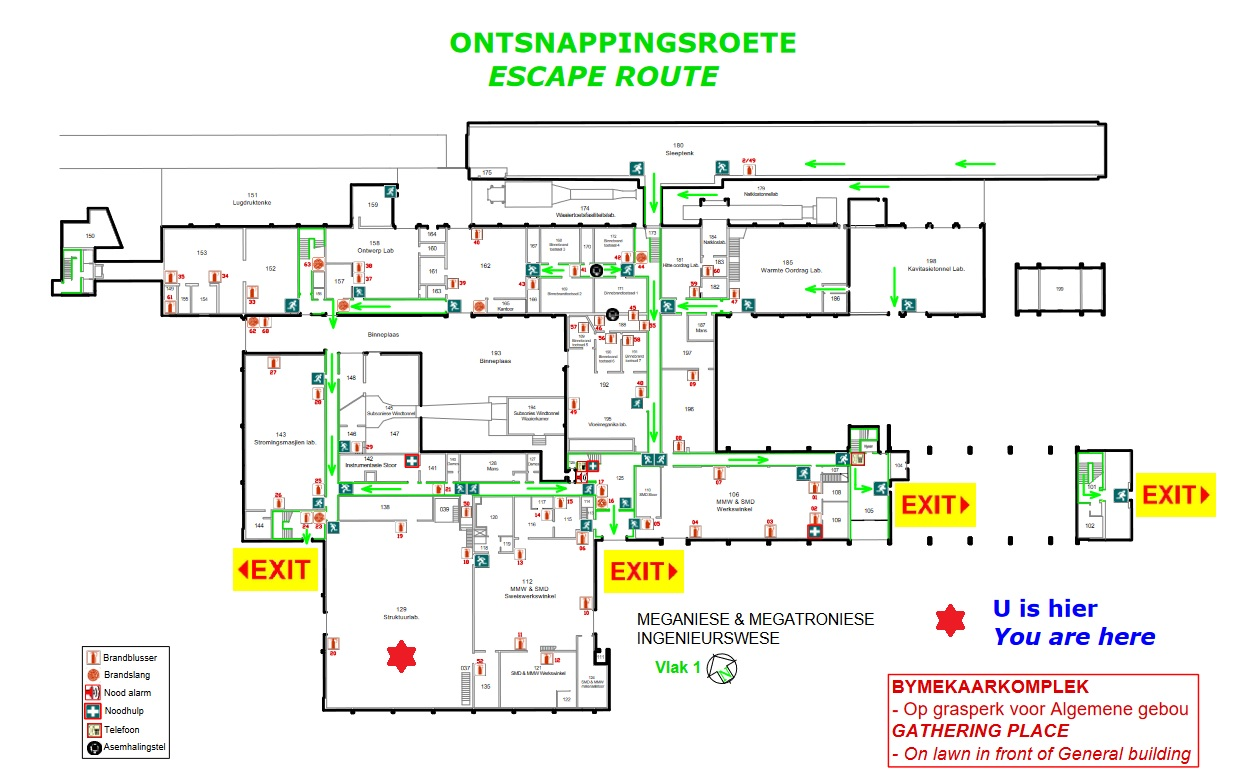
\includegraphics[width=\textwidth]{EscapeRoute.jpg}
		\caption{Structural Lab Escape Route}
		\label{fig:safe}
	\end{center}
\end{figure}

